\documentclass[11pt]{article}
\usepackage[lmargin=2.2cm,rmargin=2.2cm,tmargin=2.2cm,bmargin=2.2cm]{geometry}
\usepackage[utf8]{inputenc}
\usepackage{moreverb}
\usepackage{listings}
\usepackage{graphicx}
\usepackage{verbatim}
\usepackage{ragged2e}
\usepackage{verbatim}
\usepackage{appendix}
\usepackage{todonotes}
\usepackage{algcompatible}
\usepackage{amssymb}
\usepackage{algorithm}
\usepackage{amsmath}
\usepackage[noend]{algpseudocode} 
\setlength{\parindent}{0pt}
\usepackage{float}
\linespread{1.5}
\usepackage{framed}
\usepackage{enumitem}
\usepackage{tikz}
\usetikzlibrary{automata, arrows}
\usepackage{logicproof}
\DeclareGraphicsExtensions{.pdf,.png,.jpg}
\renewcommand*\contentsname{Summary}
\pagenumbering{arabic}
\usepackage[normalem]{ulem}
\usepackage{minted}
\usepackage{svg}
\usepackage{graphicx}


\usepackage{xcolor}
\usepackage{listings}
\definecolor{mGreen}{rgb}{0,0.6,0}
\definecolor{mGray}{rgb}{0.5,0.5,0.5}
\definecolor{mPurple}{rgb}{0.58,0,0.82}
\definecolor{backgroundColour}{rgb}{0.95,0.95,0.92}
\def\code#1{\texttt{#1}}

\lstdefinestyle{CStyle}{
    backgroundcolor=\color{backgroundColour},   
    commentstyle=\color{mGreen},
    keywordstyle=\color{magenta},
    numberstyle=\tiny\color{mGray},
    stringstyle=\color{mPurple},
    basicstyle=\footnotesize\ttfamily,
    breakatwhitespace=false,         
    breaklines=true,                 
    captionpos=b,                    
    keepspaces=true,                 
    numbers=left,                    
    numbersep=5pt,                  
    showspaces=false,                
    showstringspaces=false,
    showtabs=false,                  
    tabsize=2,
    language=C
}

\lstdefinestyle{PYstyle}{
    backgroundcolor=\color{backgroundColour},   
    commentstyle=\color{mGreen},
    keywordstyle=\color{magenta},
    numberstyle=\tiny\color{mGray},
    stringstyle=\color{mPurple},
    basicstyle=\footnotesize\ttfamily,
    breakatwhitespace=false,         
    breaklines=true,
    captionpos=b,                    
    keepspaces=true,                 
    numbers=left,                    
    numbersep=5pt,                  
    showspaces=false,                
    showstringspaces=false,
    showtabs=false,                  
    tabsize=2,
    language=Python
}




\begin{document}
	
\title{Project in Bioinformatics \\
{\scriptsize Bioinformatics Research Centre (BiRC)\vspace{-7mm} \\
AARHUS UNIVERSITY} \\
\vspace{5mm}
\textbf{Algorithmic Engineering of Hidden Markov Models}}
\author{
    \textbf{Carl M. Kobel} \\ Student ID: 201404379
    \vspace{3mm} \\
    \textbf{Thor B. Jakobsen} \\ Student ID: 201404985
    \vspace{10mm} \\
    \includegraphics[width = 70mm]{figures/ausegl_sort.png}
}

\clearpage
\maketitle
\thispagestyle{empty}

\newpage
\pagenumbering{Roman}
\setcounter{page}{1}
\tableofcontents

\newpage
\pagenumbering{arabic}
\setcounter{page}{1}

% Introduction
\section{Introduction}
Hidden Markov Models\cite{baum1966} are a group of powerful probabilistic models for modeling sequential data with a hidden underlying structure. They are widely used in the field of bioinformatics for gene finding and gene prediction. The reason for their popularity lies in their accuracy, robustness and simplicity.
When analyzing larger quantities of data with an increasingly complex underlying structure, the efficiency of Hidden Markov Models is a limiting factor. This limiting factor is rooted in the algorithms used for evaluating, decoding and training the Hidden Markov Models. All algorithms except the Viterbi algorithm rely strongly on the efficiency of two main algorithms: the Forward and the Backward algorithms.
In this report we propose a solution to the efficiency problem of Hidden Markov Models by optimizing the Forward and the Backward algorithms using linear algebra. Our solution is implemented in two libraries, one for the $C$ programming language and one for the $Python$ programming language utilizing the implementations in the $C$ library.
%Nej det er en paper convention hvor beskrivelsen af resten af rapporten er i lille da den enligt ikke er en del af introduktionen.

{\small The rest of this report is structured as follows: We will give an introduction to Hidden Markov Models and their associated algorithms in \textbf{section \ref{sec:HMM}}. Then we will present our optimizations of the Forward and the Backward algorithms in \textbf{section \ref{sec:ForwardBackward}}. Then we will present our library and its underlying architecture in \textbf{section \ref{sec:hmmmlib}}. Then we will present our results from conducting experiments with our library and see if we achieved a speed up compared to a conventional implementation in \textbf{section \ref{sec:expriments}}. We will finish the report with a conclusion in \textbf{section \ref{sec:conclusion}}.}



\section{Hidden Markov Models}\label{sec:HMM}

In the following we will introduce the Hidden Markov Model and the three basic problems of Hidden Markov Models: the evaluation problem, the decoding problem and the learning problem.

\subsection{A Hidden Markov Model}

A Hidden Markov Model (HMM) is a probabilistic model which in its simplest form consists of $M$ observables:
$$O = \{o_1\cdots o_M\}$$\

$N$ hidden states which are non observables:


$$H= \{h_1\cdots h_N\}$$

$N$ initial probabilities of starting in one of the $N$ hidden states:
$$\pi = \{\pi_1\cdots\pi_N\}$$

A $ N \times N $ transition matrix $\varphi$ where $\varphi_{i,j}$ is the probability of transitioning from state $h_i$ to state $h_j$. A $ N \times M $ emission matrix $\theta$ where $\theta_{i,j}$ is the probability to observe the $i$'th observable $o_i$ at the state $h_j$. 

\subsection{Evaluation problem}

The evaluation problem of an HMM is: Given an HMM $\lambda$ and a sequence of observations $Y$, what is the probability of observing the sequence $Y$ with respect to $\lambda$? This problem can be solved using the Forward and the Backward algorithms.

\subsubsection{Forward algorithm}\label{sec:forward}

The Forward algorithm\cite{Bishop} given a sequence of observations $Y$ of length $K$ and an HMM $\lambda$ creates an $ N \times K$ matrix $\alpha$. Here $\alpha_{i,j}$ is the probability of $\lambda$ emitting the subsequence $Y_{1:i}$ of $Y$ starting from the first observation, to the $i$'th observation and being in the $j$'th hidden state. $\alpha$ is calculated recursively in a forward manner starting from the first observation of $Y$. 
The initial step of the Forward algorithm is given by:
$$\alpha_{1,j} = \pi_j\cdot\theta_{Y_1,j}$$

The $j$'th index of the $i$'th observation of $Y$, $Y_i$, in $\alpha$ is defined as the following summation: 
\begin{align*}
    \alpha_{i,j} &= \sum\limits_{l=1}^{N} \theta_{Y_i,j}\cdot\varphi_{l,j}\cdot\alpha_{i-1,l}
\end{align*}

The Forward algorithm does $ N $ operations for each index in $\alpha$ so the overall running time is $\mathcal{O}( N ^2\cdot K)$. It uses $\mathcal{O}( N \cdot K)$ space as it fills up the $\alpha$ matrix.

\subsubsection{Backward algorithm}

The Backward algorithm\cite{Bishop} given a sequence of observations $Y$ of length $K$ and an HMM $\lambda$, creates an $ N \times K$ matrix $\beta$. Here $\beta_{i,j}$ is the probability of $\lambda$ emitting the sub-sequence $Y_{i+1:K}$ starting in the $j$'th hidden state: $P(Y_{i+1:K}|X_i = x_j)$. 
$\beta$ is calculated recursively in a backward manner starting with the last observation of $Y$ where the first row of $\beta$ has the value $1$.
\begin{align*}
    \beta_{i,j} &= \sum\limits_{l=1}^{N} \beta_{i+1,l}\cdot\varphi_{l,j}\cdot\theta_{Y_{i+1},j}
\end{align*}

Like the forward algorithm, The Backward algorithm does $ N $ operations for each index in $\beta$ so the overall running time is $\mathcal{O}( N ^2\cdot K)$. It uses $\mathcal{O}( N \cdot K)$ space as it fill up the $\beta$ matrix.

\subsection{Decoding problem}

The decoding problem of an HMM is: Given an HMM $\lambda$ and a sequence of observations $Y$, what is the most likely sequence of hidden states that produced $Y$ with respect to $\lambda$? 

\subsubsection{Viterbi algorithm}

The Viterbi algorithm\cite{Bishop} is a maximum-likelihood algorithm that, given an HMM $\lambda$ and a sequence of observations $Y$ of length $K$ computes the most likely sequence of hidden states $X = x_1,\ldots,x_K$ that generates $Y$. 
The Viterbi algorithm fills out a $K \times N$ table $V$, where $V_{i,j}$ is the probability of the most likely path ending in the $x_j$ at time $j$, having observed the subsequence $Y_{1:i}$.

$$V_{i,j} = \max\limits_{x_{j-1}} P(Y_{1:i}, X_{j+1} = x_{j+1}|\lambda)$$

The most likely sequence of hidden states can then be calculated by backtracking through $V$ starting in $\max(V_K)$.

Because the algorithm fills out a $ K \times  N $ table, where we for each cell have to iterate through all $ N $ states to find the transition with the highest probability, the running time is $\mathcal{O}(K \cdot  N ^2)$. The space consumption of the table $V$ is $\mathcal{O}(K \cdot  N )$.

\subsubsection{Posterior decoding algorithm}

The Posterior decoding algorithm\cite{Bishop}, given an HMM $\lambda$ and a sequence of observations $Y$ of length $K$, calculates an array $Z$ of size $K$ which contains the highest a posteriori probability for each observation in $Y$. 
$Z$ is calculated using the forward and backward probabilities. Here the $j$'th entrance in $Z$ is given by:

$$Z_j = \max\limits_{i\in H} (\frac{\alpha_{i,j}\cdot\beta_{i,j}}{P(Y|\lambda)})$$

Because the Posterior decoding algorithm relies on the forward and backward probabilities, its time consumption for calculating these is $\mathcal{O}( N^2\cdot K)$ and the space consumption for the $\alpha$ and $\beta$ tables are $\mathcal{O}( N\cdot K)$. If we assume that both $\alpha$ and $\beta$ are given, then the algorithm will use $\mathcal{O}( N\cdot K)$ time and $\mathcal{O}(K)$
space.

Posterior decoding and Viterbi is similar in that they, given a sequence of observables, both find a likely sequence of hidden states. The difference is that Viterbi finds the maximum likelihood sequence of hidden states over the full sequence $Y$, whereas Posterior decoding finds sequence of hidden states that gives the highest probability on the immediate observable $y_i$.

\subsection{Learning problem}

The learning problem is: Given an HMM $\lambda$ and a sequence of observations $Y$, how should the $\varphi$, $\theta$ and $\pi$ variables be adjusted so we maximize $P(Y|\lambda)$? This problem can be solved using the Baum-Welch algorithm.

\subsubsection{Baum-Welch algorithm}

The Baum-Welch \cite{Bishop} algorithm is an expectation maximization algorithm. Given a sequence of observations $Y$ of length $K$ and an HMM $\lambda$ the Baum-Welch algorithm trains the $\varphi$, $\theta$ and $\pi$ of the HMM so that the likelihood of $P(Y|\lambda)$ is a local maximum. This is done in an iterative procedure for a fixed amount of iterations or until the likelihood converges. In each iteration the algorithm updates the variables of the HMM using the forward and backward probability.

Because Baum-Welch uses the forward and backward probabilities it has to use the Forward and the Backward algorithms which both run in $\mathcal{O}( N ^2\cdot K)$ time. Updating the variables can be done with simple summations such that the overall running time is $\mathcal{O}( N ^2\cdot K)$ and uses $\mathcal{O}( N \cdot K)$ space.

% HMM and speeding them up using linear algebra
% Section on matrix multiplication
\section{Speeding up using matrix multiplications}\label{sec:ForwardBackward}

Our main observation during this project is that Baum-Welch and Posterior Decoding depend on the Forward and Backward algorithms. Looking closely at their structures they both run the Forward and the Backward algorithms, other than that, it only does one loop over the total length of the input without any computationally heavy operations. Our hypothesis is that if the efficiency of the Forward and Backward algorithms is increased, there will be an equal increase in the efficiency of the Baum-Welch and Posterior Decoding algorithms.

\subsection{Linear algebra formulations of the Forward and Backward algorithms}

The reason for formulating the Forward and the Backward algorithms using linear algebra is that it allows the implementations to take advantage of fast low level operations of the computer like SIMD.

Formulating the algorithms using linear algebra corresponds to generalizing the summations of the algorithms into matrix multiplications. While doing so we came up with a new matrix for replacing the emission and transition matrix in the context of the Forward and the Backward algorithms called the emission-transition matrix (ETM). In the following section we go through this generalization and show how the ETM is derived.

\subsubsection{Forward algorithm}
The following is the definition of $\alpha_{i,j}$ as described in \textbf{section \ref{sec:forward}}:
\begin{align}\label{forward:summation}
  \alpha_{i,j} &= \sum\limits_{l=1}^{N} \theta_{Y_i,j}\cdot\varphi_{l,j}\cdot\alpha_{i-1,l}
\end{align}

Instead of having a definition for each index of $\alpha$ we made a formulation for each column of $\alpha$. Let $\Theta_{Y_i}$ denote the diagonal matrix made from the $i$'th row in $\theta$. We use that $\Theta_{Y_i}\cdot\varphi$ results in a matrix where each row contains the same values as each iteration of the corresponding summation from \textbf{(\ref{forward:summation})}. Using this observation we can now define the $i$'th column of $\alpha$ as: %in $\theta_{Y_i,j}\cdot\varphi_{l,j}$ for $l=1\cdots|\varphi|$:
\begin{align}\label{forward:matrixmulti}
  \alpha_{i} &= \Theta_{Y_i}\cdot\varphi\cdot\alpha_{i-1}
\end{align}
We notice that we in equation \textbf{(\ref{forward:matrixmulti})} do a matrix-matrix multiplication, $\Theta_{Y_i}\cdot\varphi$, for each observation in the sequence $Y$. This can be avoided by introducing the ETM as $\hat{\Theta}_{Y_i} = \Theta_{Y_i}\cdot\varphi$. We avoid the matrix matrix multiplication because we can compute all the $ M $ ETMs as a preprocessing step so that for any $Y$ of length $K$ where $K>M$ the ETMs reduce the amount of matrix matrix multiplications compared to \textbf{(\ref{forward:matrixmulti})}. Using the definition of the ETM we can now define the $i$'th column of $\alpha$ as:
\begin{align}\label{forward:final}
  \alpha_i &= \hat{\Theta}_{Y_i}\cdot\alpha_{i-1}
\end{align}

It is not possible to use the ETM in the initial step of the forward algorithm but it can still be described using linear algebra using the $\Theta_{Y_{1}}$ from \textbf{(\ref{forward:matrixmulti})}:
\begin{align*}
  \alpha_{1} &= \pi\cdot\Theta_{Y_{1}}
\end{align*}

\subsubsection{Backward algorithm}

The initial step of the Backward algorithm cannot be meaningfully described with linear algebra since no operations are made. However the $i$'th step can and we will introduce the notation of ETM for the $i$'th step of the backward algorithm. The $i,j$'th index of $\beta$ is defined as:
\begin{align*}
  \beta_{i,j} &= \sum\limits_{l=1}^{N} \beta_{i+1,l}\cdot\varphi_{j,l}\cdot\theta_{Y_{i+1},j}
\end{align*}

We now introduce $\Theta_{Y_{i+1}}$ from \textbf{(\ref{forward:matrixmulti})} and write $i$'th column of $\beta$ as:
\begin{align*}
  \beta_i = \beta_{i+1}\cdot\varphi\cdot\Theta_{Y_{i+1}}
\end{align*}

Finally we introduce the ETM into the definition of the $i$'th column of $\beta$:
\begin{align}\label{beta:one}
  \beta_{i} &= \beta_{i+1}\cdot\hat{\Theta}_{Y_{i+1}}
\end{align}
        
\subsubsection{Increased space consumption}

The ETM matrix has the dimension $N \times N$ and since there are $ M $ of them, we get a space consumption increase of $\mathcal{O}(M \cdot N^2)$.

\subsubsection{Sparse matrix}

Because we introduced the linear algebra formulation of the Forward and the Backward algorithms the instances where the emission or the transition matrix is sparse should be addressed. A sparse matrix is a matrix where most of the elements are zero, which means doing vector matrix multiplication most of the multiplications will have the form: 

$$A\cdot x = a_{i,1}\cdot x_1\cdots a_{i,n}\cdot x_n = 0\cdot x_1\cdots0\cdot x_n$$

It is clear that these multiplications are trivial. Our hypothesis is that in these instances it is possible to achieve an even greater speed up than expected for the straight forward linear algebra implementation. 
First of all we see that the ETMs are sparse when the transition matrix or the emission matrix is sparse. This means only one of the matrices have to be sparse before we consider our instance to be sparse. It is possible to represent a sparse matrix on a format where all zero values are omitted. If such a format allows for vector matrix multiplications it can be used for representing the ETM. There exist many different sparse matrix formats that support matrix vector multiplication. We choose to focus on the Compressed Sparse Row (CSR) format and the Recursive Sparse Block (RSB) format. 


\subsection{Implementation}\label{sec:impel}

In the following section we will go though the main points of our implementations of the Forward and the Backward algorithms with respect to the dense and sparse instance of the ETM.

\subsubsection{BLAS}\label{sec:blas}
BLAS\cite{blackford2002updated} stands for basic linear algebra subprograms. It is a specification that describes a set of routines for performing basic linear algebra operations. BLAS is typically implemented so that it is optimized for specific hardware. The major vendors like AMD\cite{amd} and Intel\cite{intel} have their own implementation optimized for their own CPUs. BLAS is the de facto specification for linear algebra operations which is the reason why we choose it for implementing our linear algebra formulation of the Forward and the Backward algorithms. We chose the ATLAS\cite{ATLAS} distribution which complies so that it is optimized for the hardware it is compiled on.


The following code snippet performs the calculation of the $i$'th column of $\alpha$ as described in \textbf{equation (\ref{forward:final})} using BLAS. In this step only one matrix vector multiplication is necessary. This is done by using the \texttt{cblas\_dgemv} function. \texttt{cblas\_dgemv} computes \texttt{y := alpha*A*x + beta*y} or where \texttt{A} is transposed depending on the input. In the following code we perform the transposed version. To achieve just the \texttt{y := A*x} part we set \texttt{alpha=1}, \texttt{beta=0} and \texttt{y} is a pointer to the beginning of the $i$'th column of $\alpha$. We transpose the \texttt{A} (ETM) because it is stored in transpose order in the implementation and transposing it again moves it back.


\begin{lstlisting}[style=CStyle]
cblas_dgemv(CblasRowMajor, CblasTrans, hmm->hiddenStates, hmm->hiddenStates, 1.0, new_emission_probs[Y_i], hmm->hiddenStates, alpha+hmm->hiddenStates*(i-1), 1, 0, alpha+hmm->hiddenStates*i, 1);
\end{lstlisting}


The following code snippet performs the calculation of the $i$'th column of $\beta$ using BLAS. Here we do the same as previous code but where we use the first, untransposed, version. Because we want to perform a vector matrix multiplication as denoted in \textbf{(\ref{beta:one})}, but \texttt{cblas\_dgemv} only allows us to do a matrix vector multiplication, we benefit form the ETM being quadratic. By transposing the ETM and then doing a matrix vector multiplication makes it the same as doing a vector matrix multiplication. As the ETM is transposed by default we do nothing.
\begin{lstlisting}[style=CStyle]
cblas_dgemv(CblasRowMajor, CblasNoTrans, hmm->hiddenStates, hmm->hiddenStates, 1.0, new_emission_probs[Y[T-i]], hmm->hiddenStates, beta+hmm->hiddenStates*T-i*hmm->hiddenStates, 1, 0, beta+hmm->hiddenStates*T-i*hmm->hiddenStates-hmm->hiddenStates, 1);
\end{lstlisting}

We can also calculate the ETM's using BLAS which we did.

\subsubsection{CSR}\label{sec:csr}

The CSR format represent a sparse matrix using three arrays. One that contains all the non zero values of the matrix and two arrays for keeping track of the value indices in the original matrix. The format allows for vector matrix multiplication. The implementation utilizing the CSR format has a larger preprocessing as we have to calculate the ETMs and then turn them into the CSR format. The matrix vector multiplication using the CSR format consists of two nested loops that goes through the two index arrays. The amount of iterations in the loops and therefore the amount of multiplications are bounded by the amount of non-zero values in the ETM. The implementation uses BLAS for calculating the ETM's.

\subsubsection{RSB}
There is no straight forward implementation of sparse matrix vector multiplication utilizing low level operations of the computer like there is with BLAS. Instead we found libRSB\cite{librsb}, a library that implements the sparse BLAS specifications, which is a subset of the original BLAS operations for sparse matrix operations. The implementation takes advantage of the recursive sparse block matrix format that allows for cache efficient and multi threaded matrix operations. We use the libRSB as shown in the code snippet in \textbf{section (\ref{sec:blas})} the corresponding libRSB function is called \texttt{rsb\_spmv}. The \texttt{rsb\_spmv} function takes the same parameters however the input matrix must be in CSR format. Therefore the implementations of the Forward and the Backward algorithms for the sparse instance of  an HMM utilizing RSB has the same preprocessing step as the CSR version described in \textbf{section (\ref{sec:csr})}. The implementation uses BLAS for calculating the ETM's.

\subsection{Scaling}
In order to avoid the numerical problems associated with multiplying probabilities (or numbers smaller than 1) we have to scale the results for each iteration of the Forward and the Backward algorithms. For the Forward algorithm we divide each cell in the current column with its sum. The sum was then saved in the \texttt{scaleFactor} variable to be used for scaling the Backward algorithm. To obtain compatible scaling, we use the same scale factor for the Forward algorithm when scaling the Backward algorithm, as in: we divide each cell with the sum of the corresponding column of the result of the Forward algorithm. 

The scaling step can be done in two lines when using BLAS, which we did for both the BLAS, CSR and RSB implementations. The conventional implementation of the Forward and Backward algorithms is scaled using a single loop.



% Creating a Library ... Section on python-binding
\section{HMMM (Hidden Markov Model Matrix{\small\textit{-edition}})}\label{sec:hmmmlib}

In the following we will go though our main software architectural considerations about our \texttt{C} implementation of the HMM and its algorithms as well for the associated \texttt{Python} library. Both the \texttt{C} library and the \texttt{Python} library can be found on the Hidden Markov Model Matrix-edition github at: \code{https://github.com/Thornado-Carlkoder/hmmmlib}

\subsection{C implementation}

Our \texttt{C} implementation of the HMM and its associated algorithms are strongly influenced by our experimental implementations of the Forward and the Backward algorithms. We wanted our implementation to facilitate easy switches between implementations of the Forward and the Backward algorithms as well as ensuring that these implementations could be compared on the same basis.

To encapsulate the HMM we made a \texttt{struct} which contains the variables of the HMM as described in \textbf{section (\ref{sec:HMM})} as well as the size of its variables. The struct is shown on \textbf{figure \ref{fig:hmmstruct}}.
\begin{figure}[H]
    \centering
    \begin{lstlisting}[style=CStyle]
    struct HMM {
        unsigned int hiddenStates;
        unsigned int observations;
        double * transitionProbs;
        double * emissionProbs;
        double * initProbs;
        void (*forward)(struct HMM *hmm, const int *Y, const int T, double * scalingFactor, double * alpha);
        void (*backward)(struct HMM *hmm, const int *Y, const int T, double * scalingFactor, double * beta);
    };\end{lstlisting}
    \caption{Struct of the HMM in the \texttt{C} implementation}
    \label{fig:hmmstruct}
\end{figure}
All the algorithms are implemented so the user is in charge of allocating and deallocating all the output variables. For each algorithm, a pointer to the output must be given as a parameter. This is done to give the user as much control as possible.
To allow an easy way of changing implementations of the Forward and the Backward algorithms, and to avoid multiple implementations of the Baum-Welch and the Posterior decoding algorithms, we made an interface for both the Forward and the Backward algorithms. These are added to our HMM struct as two function pointers and are the last two variables of \textbf{figure \ref{fig:hmmstruct}}. This allows us to call the two algorithms through the HMM instance which is a required argument in the Baum-Welch and the Posterior decoding algorithms. This allows these algorithms to call the Forward algorithm like this:
\begin{lstlisting}[style=CStyle]
F(hmm, Y, T, scaleFactor, alpha);\end{lstlisting}

The Backward algorithm can be called in the same manner. 
This made it very easy to construct a new version of the Forward and the Backward algorithms since they just need to follow the interface. To simplify this even more we made HMM constructors for the different versions of the Forward and Backward algorithms so the different constructors set the function pointers to the wanted implementations of the Forward and the Backward algorithms.

The following code snippet is an usage example of the \texttt{C} library:

\begin{figure}[H]
    \centering
    \begin{lstlisting}[style=CStyle]
    HMM * hmm = HMMBLAS(7, 4);
    double transitionProbs[7][7] = {
     {0.0, 0.0, 0.9, 0.1, 0.0, 0.0, 0.0},
                        ...
     {0.0, 0.0, 0.05, 0.9, 0.0, 0.05, 0.0},
    };
    double emissionProbs[4][4] = {
     {0.3, 0.25, 0.25, 0.2},
                ...
     {0.25, 0.25, 0.25, 0.25},
    };
    double initProbs[7] = {0.0, 0.0, 0.0, 1.0, 0.0, 0.0, 0.0};
    int input[1000] = {0, 2, 1, 1, ..., 3, 2, 2};
    double * alpha = malloc(1000*hmm->hiddenStates*sizeof(double));
    double * scaleFactor = malloc(1000*sizeof(double));
    F(hmm, input, 1000, &scaleFactor, &alpha);
    HMMDeallocate(hmm);\end{lstlisting}
    \caption{In the \texttt{C} library example we initialize the BLAS version of the HMM with 7 hidden states and a alphabet of size 4. We set its transition, emission and initial probabilities. When these a set the HMM instance is ready to be used. From line 13 to 16 we make a alpha pointer and a scale factor pointer and then call the Forward function of the HMM where the result is saved to the alpha pointer. At line 17 we end our example by  deallocating the HMM struct and its pointers.}
    \label{fig:c_example}
\end{figure}


\subsubsection{Implementation of Baum-Welch, Posterior decoding and Viterbi}

To get a complete library with the HMM and it's associated algorithms and being able to test our hypothesis we implemented the Baum-Welch, Posterior decoding and Viterbi algorithms in a conventional manner without doing any optimization.
% \todo{forslag: In order to have a benchmark for our hypothesized optimizations, we created an HMM-library, containing a conventional implementation of all the algorithms.}

The Baum-Welch and Posterior Decoding algorithms both take advantage of the Forward and Backward algorithms. Thus they were implemented using the interface described in the previous section for calling the Forward and the Backward algorithms.

The Viterbi algorithm is scaled using logarithm in order to avoid numerical problems. We tested our implementation of the Viterbi algorithm to validate that it has the expected running time, which it has. The result of the experiment can be seen on \textbf{figure \ref{app:viterbi}} in the Appendix. 

We also tested all the algorithms scale accordingly with respect to the state space, which they do. The results of theses experiments are shown on \textbf{figure \ref{app:hiddenstates}} in the Appendix.

\subsection{Python library}\label{sec:pb}
To make the HMM-library easily accessible, in order to quickly write tests, we decided to write a Python library which makes it possible to call all core methods and algorithms in the \texttt{C}-library.

The Python library is constructed by compiling the \texttt{C} library into a shared object which is then loaded into Python using the ctypes\cite{ctypesman} foreign function library for Python.
This is done in the Python file \code{HMMM.py}.
In the main file of the Python library, the HMM-struct and all of it's functions and algorithms are defined. By importing this library, all the functions and algorithms in the C-library will be accessible in Python.
% To ensure that the library works as expected we made a test, that imports this library, and verifies that all algorithms produce correct outputs for defined inputs. 
Each time a new function or algorithm is added to the C-library, a corresponding definition must be made in HMM.py.

In the Python library, we implemented the \texttt{\_\_del\_\_(self)} data model method\cite{pythonman}, so when the reference count of the Python HMMM-class object reaches zero, the C-library actively deallocates all dynamically allocated memory. When using the python binding no manual data management is needed.

The following is an example of how to use the python library:

\begin{figure}[H]
    \centering
\begin{lstlisting}[style=PYstyle]
from HMMM import *
hmmm = HMMM(3, 2, hmmType = "BLAS") 
hmmm.set_random()  
hmmm.setInitProbs([1,0,0])
hmmm.baumWelch(observations = [1,0,1,0,1,0,1,...,1,0,1,1,0,1,0,1], n_iterations = 5)\end{lstlisting}
\caption{\small{Example of the python library. Setting up an HMM with 3 hidden states and an alphabet of size 2 using the BLAS-implementation. At line 3 the initialization, emission and transition matrices are set to random values. At line 4 the initialization probabilities is set to a specific list of values.
At line 5 the Baum-Welch algorithm is used to train the transition and emission matrices using given data over 5 iterations.}}
\label{fig:pybind}
\end{figure}

\subsubsection{Running time tests}\label{sec:runningtimetests}
We performed running time tests on all algorithms using the Python library. All the tests where made using uniform randomly generated strings made over the alphabet as input. We used the same input for every version of the different algorithms.

The advantage of using the Python library is that it was very easy to modify the tests and automate them. The disadvantage is that it introduces a level of abstraction, thereby possibly adding noise to the time measurements.

% \subsection{Python binding}\label{sec:pb}
% In order to make the HMM-library easily accessible from an abstract programming environment - such that we could easily write tests - we decided to write a Python binding that makes it possible to call all core methods and algorithms in the C-library.

% The hmm-library written in \code{C} compiled to a shared object. In binding.py, this shared object is loaded into python using the ctypes-library. Here, the structure of the HMM-struct and all of its functions and algorithms are defined. By importing this binding, alle the functions and algorithms in the C-library will be accessible in Python. We have made a test, that imports this binding, and verifies that all algorithms are indeed callable and that they produce correct outputs for defined inputs. Each time a new function or algorithm is added to the HMM-library written in C, a corresponding definition must be made in binding.py.
% The usage of the python binding is exemplified in \textbf{figure \ref{fig:pybind}}.

% In the Python binding, we implemented the \texttt{\_\_del\_\_(self)} data model method, such that when the reference count of the Python HMMM-class reaches zero, the the C-library deallocates all dynamically allocated memory.

% \todo{Jeg tror at beskrivelsen af koden er i passiv stemme?! C: Kigger lige på det.}
% \begin{figure}[H]
%     \centering
% \begin{lstlisting}[style=PYstyle]
% from binding import *

% hmmm = HMMM(3, 2, hmmType = "BLAS")
% hmmm.set_random()
% hmmm.setInitProbs([1,0,0])

% hmmm.baumWelch(observations = [1,0,1,0,1,0,1,...,1,0,1,1,0,1,0,1],
%       n_iterations = 5)\end{lstlisting}
% \caption{\small{Python binding practical example. Setting up an HMM with 3 hidden states and an alphabet size of 2 using the BLAS-implementation. Setting up the initialization, emission and transition matrices to random values as well as changing the initialization probabilities to a specific list of values. Then applying the Baum-Welch algorithm to train the transition and emission matrices to given data with 5 iterations.}}
% \label{fig:pybind}
% \end{figure}



% \subsubsection{Running time tests}\label{sec:runningtimetests}
% We performed running time tests on all algorithms through the Python binding. All tests have a precisely defined number of hidden states, alphabet size, length of input, number of replicates etc. The input of observables to the algorithms is in all cases a uniform random generated string under the alphabet size. The benefit of using the Python binding to perform the running time tests is that it is easy to define and edit these tests, the disadvantage is that noise might be introduced in the time measurement.


% Section on experiments etc.
\section{Experiments}\label{sec:expriments}
To test or hypotheses we have conducted several experiments on the different implementations of the Forward and the Backward algorithms. All the experiments have been conducted on a ThinkPad W540 with 32GB RAM and an Intel I7-4700MQ running 64bit Debian 10. The \texttt{C}-library was written in \code{C} version 11 and compiled using \texttt{gcc} version 8.3.0-6. We used \texttt{Python} version 3.7.3. All the experiments have 3 replicates in order to minimize random fluctuations due to other processes of the computer.
All experiments were conducted through the \texttt{Python}-library as described in \textbf{section \ref{sec:pb}}.

\subsection{BLAS vs Conventional}\label{sec:A1}
To test our initial hypothesis, that a linear algebra implementation utilizing BLAS of the Forward and the Backward algorithms is faster than the conventional version, we conducted the following experiment.

The experiment was conducted with an varying input size starting with $100'000$ going up to $1'000'000$, increasing $100'000$ each time. The state space was varied as well: from $10$ to $400$. Varying the state space allows us to test the consistency of the performance over all the influencing variables. The experiment is show in \textbf{figure \ref{fig:A1}}. 

\textbf{Figure \ref{fig:A1}} clearly shows that the BLAS version is faster than the conventional implementation in all experiments. It is also clear that the efficiency ratio between the BLAS version and the conventional implementation increases with the size of the state space. This supports our initial hypothesis. 

\begin{figure}[H]
  \centering
  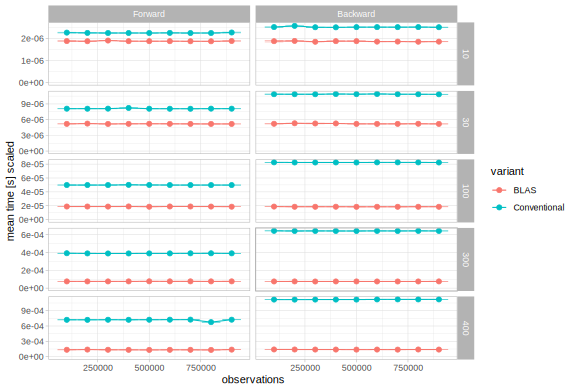
\includegraphics[scale=0.85]{figures/figure_A1.pdf}
  \caption{\small{Forward and Backward running time experiment for the linear algebra and the conventional implementations. The vertical axis shows time divided by number of observations. Error bars denote standard deviation of 3 replicates. Alphabet size: 4.}}
  \label{fig:A1}
\end{figure}

To verify that the algorithms scale with their theoretical running times the measured time is divided with the input size on \textbf{figure \ref{fig:A1}}. It is clear that the algorithms follow their theoretical running times for both implementations.

\textbf{Figure \ref{fig:A1}} implies that the BLAS implementation is faster than the conventional implementation supporting our hypothesis. This is especially clear when the state space increases.

\subsubsection{Baum-Welch and Posterior decoding}\label{sec:A2}

In the following experiment we want to test our hypothesis, that if we increase the speed of the Forward and the Backward algorithms we will see an equal speed up in the Baum-Welch and the Posterior decoding algorithms. \textbf{Figure \ref{fig:A2}} shows the experiment running the Baum-Welch and the Posterior decoding algorithms using the conventional and BLAS version of the Forward and the Backward algorithms.

\begin{figure}[H]
  \centering
  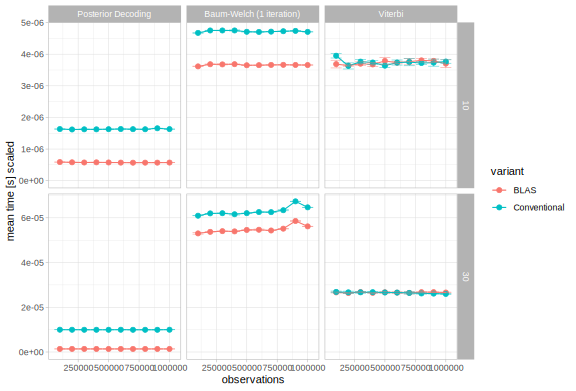
\includegraphics[scale=0.85]{figures/figure_A2.pdf}
  \caption{\small{Posterior decoding and Baum-Welch running time experiment with the BLAS version and the conventional implementation. The vertical axis shows time divided by number of observations. Error bars denote standard deviation of 3 replicates. Alphabet size: 4.}}
  \label{fig:A2}
\end{figure}

To verify that the algorithms scale with their theoretical running times, we have divided the measured time with the input size on \textbf{figure \ref{fig:A2}}. It is clear that the algorithms follow their theoretical running times for both algorithms.

\textbf{Figure \ref{fig:A2}} clearly shows that there is an equivalent increase in speed for both the Baum-Welch and Posterior decoding algorithms, supporting our hypothesis.

\subsection{Sparse instance of HMM}

To test our hypothesis for the sparse instance of an HMM, we implemented versions of the Forward and the Backward algorithm utilizing the CSR format and the RSB format as described in \textbf{section \ref{sec:impel}}. In the following two experiments we tested the two implementations against each other, and in the last experiment we tested the fastest of these (RSB) against the BLAS implementation.

We define density as a value between 0 and 1, where a density of 0 signifies the most sparse valid transition matrix where only one value per row is non-zero. 
When the density goes towards 1, the number of edges in the matrix goes from $N$ to $N^2$.

All the experiments are conducted with an input size of $100'000$ observables, whilst varying the density of the transition matrix and the state space. For all the experiments we use a dense emission matrix with $4$ observables. 

\subsubsection{RSB vs CSR}

In the following experiment compare the RSB and CSR implementations of the Forward and the Backward algorithms. The results of this experiment are shown on \textbf{figure \ref{fig:B3}}. 

\begin{figure}[H]
  \centering
  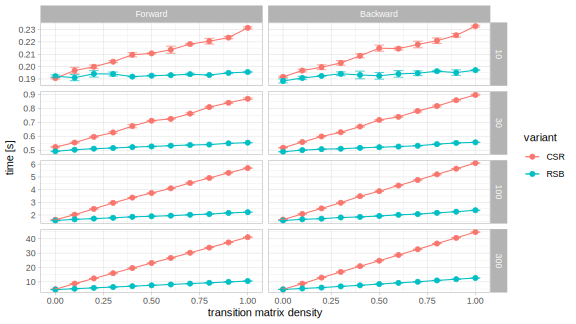
\includegraphics[scale=0.85]{figures/figure_B3.pdf}
  \caption{\small{Comparison of the two sparse implementations: CSR and RSB. Forward and Backward algorithms with a fixed input of size $100'000$ and varying state space and density. Alphabet size of 4.}}
  \label{fig:B3}
\end{figure}

From \textbf{figure \ref{fig:B3}} it is clear that the RSB implementation is faster than the CSR implementation for all combinations of state space size and density.

\subsubsection{BLAS vs RSB}\label{sec:B1}

In the following experiment we want to test our hypothesis, that the implementations of the Forward and the Backward algorithms optimized for sparse instance of an HMM utilizing libRSB yields a speed up compared to our density-ignorant BLAS version when the transition matrix is sparse.

\begin{figure}[H]
  \centering
  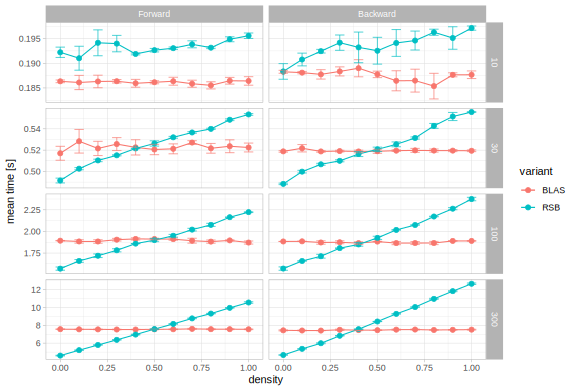
\includegraphics[scale=0.85]{figures/figure_B1.pdf}
  \caption{\small{Experiment of the BLAS and RSB implementations of the Forward and Backward algorithms with a fixed input of size $100'000$ and varying state space and density. Alphabet size of 4.}}
  \label{fig:B1}
\end{figure}

\textbf{Figure \ref{fig:B1}} shows that for the state spaces in the range of $30$ and up, the RSB implementation has a speed up relative to the BLAS version when the density is below $0.375$. This speed up goes for both the Forward and the Backward algorithms. It seems like the advantage of the Forward algorithm is stabilizing at a density of $0.5$ and for the Backward algorithm it is stabilizing at $0.375$.

This supports or hypothesis, that it is possible to achieve a speed up for the sparse instances of the HMM when utilizing the sparseness. 
The increase in speed should also be present in the Baum-Welch and Posterior decoding algorithms as implied in the results of \textbf{section \ref{sec:A2}}.

\subsection{Conclusion on experiments}
Throughout all of our experiments we have managed to support our hypotheses, that utilizing linear algebra increases the efficiency of the Forward and Backward algorithms in \textbf{section \ref{sec:A1}} and that this increase is present in the Baum-Welch and Posterior Decoding algorithms in \textbf{section \ref{sec:A2}}. We have also shown, experimentally, that utilizing the sparse implementation of matrix multiplications leads to a further increase in speed for sparse instances of the HMM in \textbf{section \ref{sec:B1}}.


% Conclusion
\section{Conclusion}\label{sec:conclusion}


In this project report we have made a linear algebra formulation of the Forward and Backward algorithms with the hypothesis that this would increase the efficiency of these to algorithms, as well as the Baum-Welch and the Posterior decoding algorithms when implemented. We have implemented these algorithms in a conventional manner and the linear algebra formulation using BLAS. With the latter we have conducted experiments that supports our hypothesis. We have also made an implementation of the Forward and the Backward algorithms which takes advantage of the sparse instances of an HMM using RSB. We have made experiments with results supporting our hypothesis that the sparse instances of an HMM allows for an even greater speed up.
From this project report and our experiments we can conclude that the linear algebra implementation of the Forward and Backward algorithms yields a significant increase in speed not only for the latter two but for all the algorithms, that uses them as an subroutine. We can also conclude that an even greater increase in speed can be achieved when the instance of the HMM is sparse.


% In this project report we have made a linear algebra formulation of the Forward and the Backward algorithms with the hypothesis that this would increase the efficiency of these to algorithms as well as the Baum-Welch and Posterior decoding algorithms when implemented. We have implemented these algorithms in a conventional manner and the linear algebra formulation using BLAS. With the latter we have conducted experiments which results support our hypothesis. We have as well made an implementation of the Forward and the Backward algorithms which takes advantage of the sparse instances of an HMM using RSB. We have made experiments with results that support our hypothesis that the sparse instances of an HMM allows for a even greater speed for the sparse optimized implementations.
% From this project report and our experiments we can conclude that the linear algebra implementation of the Forward and Backward algorithms yields a significant increase in speed not only for the latter two but for all the algorithms that use these algorithms as a subroutine. We can also conclude that an additional increase in speed can be achieved when the instance of the HMM is sparse.





\newpage

\bibliography{ref}{}
\bibliographystyle{plain}

\newpage
\appendix
\section{Appendix}


\todo{Overvej at fjerne appendiks}



% \begin{figure}[H]
%     \centering
%     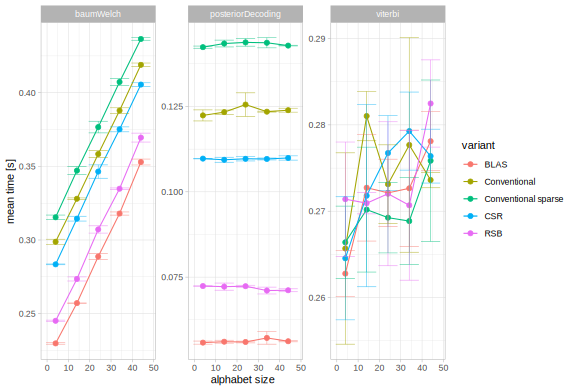
\includegraphics[scale=0.85]{figures/figure_C1.pdf}
%     \caption{Running time of increasing alphabet size for all implementations. All algorithms but Forward and Backward. Time measurement is averaged over 3 replicates. Error bars indicate standard deviation.}
%     \label{app:alphabet}
% \end{figure}


\begin{figure}[H]
    \centering
  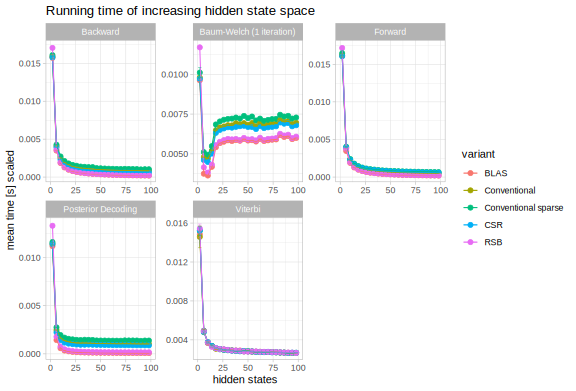
\includegraphics[scale=0.85]{figures/figure_C3_scaled.pdf}
    \caption{Running time of increasing number of hidden states for all algorithms and all implementations. Time measurement is averaged over 3 replicates. Error bars indicate standard deviation. Alphabet size = 4, input size = 100'000.}
    \label{app:hiddenstates}
\end{figure}




\begin{figure}[H]
    \centering
    \includegraphics[scale=0.85]{figures/figure_A3_scaled.pdf}
    \caption{Running time of increasing number of observations in the Viterbi algorithm. For 10 and 30 hidden states. Time measurement is averaged over 3 replicates. Error bars indicate standard deviation. Alphabet size = 4. }
    \label{app:viterbi}
\end{figure}


%\begin{figure}[H]
%    \centering
%    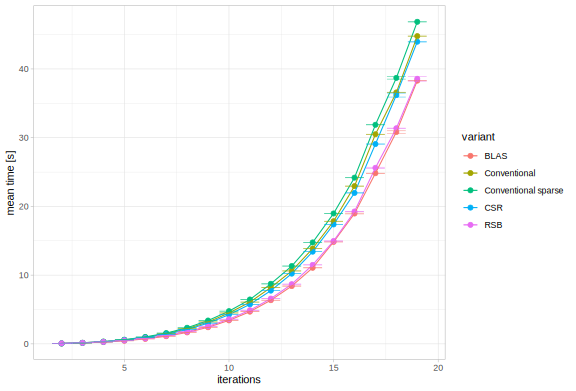
\includegraphics{figures/figure_C4_raw.pdf}
%    \caption{Running time for increasing iterations of the Baum-Welch algorithm. %Time measurement is averaged over 3 replicates. Error bars indicate standard %deviation. Alphabet size = 4, input size = 100'000 observations.}
%    \label{app:baumwelchiterations}
%\end{figure}

\end{document}
